\documentclass[11pt]{article}

% ---------- Page & fonts ----------
\usepackage[margin=1in]{geometry}
\usepackage[utf8]{inputenc}
\usepackage[T1]{fontenc}

% ---------- Math ----------
\usepackage{amsmath, amssymb, amsthm, mathtools}

% ---------- Graphs / figures ----------
\usepackage{tikz}
\usetikzlibrary{positioning, arrows.meta, calc}

% ---------- Quality of life ----------
\usepackage{enumitem}
\usepackage{hyperref}
\usepackage{cleveref}
\usepackage{xcolor}

\hypersetup{
  colorlinks=true,
  linkcolor=blue!50!black,
  citecolor=blue!50!black,
  urlcolor=blue!50!black
}

% ================= Theorem environments =================
\theoremstyle{plain}
\newtheorem{theorem}{Theorem}[section]
\newtheorem{lemma}[theorem]{Lemma}
\newtheorem{proposition}[theorem]{Proposition}
\newtheorem{corollary}[theorem]{Corollary}
\newtheorem{conjecture}[theorem]{Conjecture}

\theoremstyle{definition}
\newtheorem{definition}[theorem]{Definition}
\newtheorem{example}[theorem]{Example}
\newtheorem{exercise}[theorem]{Exercise}

\theoremstyle{remark}
\newtheorem{remark}[theorem]{Remark}
\newtheorem*{note}{Note}

% ================= Graph theory macros =================
% Sets
\newcommand{\V}{V}                       % vertex set
\newcommand{\A}{A}                       % arc set
\newcommand{\N}{N}                       % neighbourhood, N(v)

% Common graph families
\newcommand{\Kn}[1]{K_{#1}}              % complete graph K_n
\newcommand{\Kmn}[2]{K_{#1,#2}}          % complete bipartite K_{m,n}
\newcommand{\Cn}[1]{C_{#1}}              % cycle
\newcommand{\Pn}[1]{P_{#1}}              % path

% Invariants (as operators, upright text, correct spacing)
\DeclareMathOperator{\dg}{d}             % degree, use dg(v) to avoid clashing with \deg
\DeclareMathOperator{\ex}{ex}            % extremal function ex(n, H)
\DeclareMathOperator{\girth}{girth}
\DeclareMathOperator{\diam}{diam}
\DeclareMathOperator{\Aut}{Aut}
\DeclareMathOperator{\chr}{\chi}          % chromatic number, use \chr(G)
\DeclareMathOperator{\comp}{c}            % number of components

% Misc shorthands
\newcommand{\iso}{\cong}                 % isomorphic
\newcommand{\subgraph}{\subseteq}        % spanning/sub relations, adjust as needed

% ================= TikZ Styles =================
\tikzset{
    vertex/.style={
        circle,
        draw=black,
        fill=black,
        inner sep=1.8pt
    },
    edge/.style={
        thick
    },
    rededge/.style={
        thick,
        red
    },
    blueedge/.style={
        thick,
        blue
    }
}

% ================= Document =================
\title{2-d Kernels of a Digraph}
\author{Siddharth Narayan Mishra}
\date{\today}

\begin{document}

\maketitle

\section{2-d Kernel}

\begin{definition}[Independent Set]
  Let $D=(V,A)$ be a digraph. A set $S\subseteq V(D)$ is \textbf{independent} if no two vertices of $S$ are joined by an arc of $D$, i.e.\ $(u,v)\notin A(D)$ for every $u,v\in S$.
\end{definition}

\begin{definition}[2-Dominant Set]
  Let $D=(V,A)$ be a digraph. A set $S\subseteq V(D)$ is \textbf{2-dominant} if every vertex not in $S$ has at least two out-neighbours in $S$, i.e.\ for every $x\in V(D)\setminus S$,

  \[
    \left|\{y\in S: (x,y)\in A(D)\}\right|\ge 2.
  \]
\end{definition}

\begin{definition}[2-d Kernel]
  Let $D=(V,A)$ be a digraph. A subset $N\subseteq V(D)$ is a \textbf{2-d kernel} of $D$ if $N$ is both independent and 2-dominant. Equivalently, $N$ is a 2-d kernel if

  \begin{enumerate}
    \item no two vertices of $N$ are joined by an arc of $D$, and
    \item every vertex $x\in V(D)\setminus N$ has arcs into at least two distinct vertices of $N$.
  \end{enumerate}

  This is stronger than the classical (von Neumann--Morgenstern) kernel, which only requires each outside vertex to reach $N$ by \emph{some} arc; a 2-d kernel requires \emph{at least two}.
\end{definition}

\bigskip

\begin{example}
  In the digraph below, $N=\{v_1,v_3\}$ is a 2-d kernel: $v_1$ and $v_3$ are not joined by an arc, and each of $v_2,v_4$ has an arc into both $v_1$ and $v_3$, so each outside vertex has two arcs into $N$.

  \begin{center}
    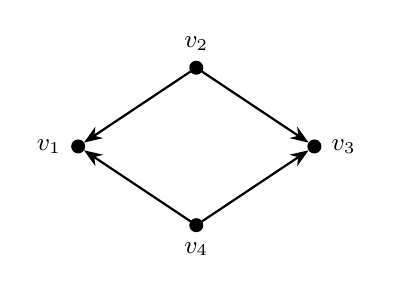
\begin{tikzpicture}[
        vertex/.style={circle, draw, fill=black, inner sep=1.5pt},
        every node/.style={font=\small},
        ->,>=Stealth,thick
      ]
      \node[vertex, label=left:$v_1$]  (v1) at (0, 0)   {};
      \node[vertex, label=above:$v_2$] (v2) at (1.5, 1) {};
      \node[vertex, label=right:$v_3$] (v3) at (3, 0)   {};
      \node[vertex, label=below:$v_4$] (v4) at (1.5, -1) {};

      \draw (v2) -- (v1);
      \draw (v2) -- (v3);
      \draw (v4) -- (v1);
      \draw (v4) -- (v3);
    \end{tikzpicture}
  \end{center}
\end{example}

\begin{remark}
  If $N$ is a 2-d kernel of $D$, then $N$ is also an ordinary kernel of $D$ (independence is unchanged, and having two arcs into $N$ certainly gives at least one). The converse fails: $N=\{v_1,v_3\}$ ceases to be a 2-d kernel if, say, the arc $v_4\to v_3$ is deleted, even though it remains an ordinary kernel as long as $v_4\to v_1$ survives.
\end{remark}

\end{document}
